% @author Marcel Ruland (2018)

%% tell TeXshop to compile using LuaLaTeX and encode with UTF-8
%!TEX TS-program = lualatex
%!TEX encoding = UTF-8 Unicode

\documentclass[
	fontsize=11,			% font size 11pt (KOMA default)
	DIV=calc,				% KOMA calculates Satzspiegel
	BCOR=0mm,				% length that will get swallowed up by binding
	pagesize,				% ensures compatibility with PDF and DVI
	toc=bib,				% include bib in toc
	toc=listof,				% include list of tables and list of figures in toc
	abstract=true,			% display abstract heading
	twoside,				% two-sided printing
	titlepage=firstiscover,	% set title page as cover page
	footnotes=multiple		% separate footnotes set directly one after another by a comma
]{scrreprt}

\usepackage{../scrreprt/ba_style}  % loading packages, typesetting, etc.

\begin{document}
\begin{figure}
	\centering
	% !TEX root = ../ba_master.tex
% @author Marcel Ruland (2018)
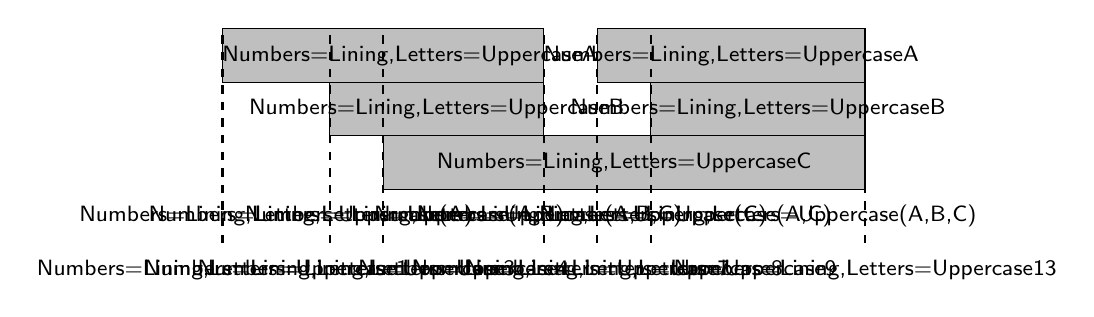
\begin{tikzpicture}[
	scale=0.68,
	every node/.append style={font=\footnotesize\sffamily\addfontfeature{Numbers=Lining,Letters=Uppercase}}]
	% boxes
	\draw [fill=lightgray] (0,4) rectangle (6,5);  % A1
	\node at (3.5,4.5) {A};
	
	\draw [fill=lightgray] (7,4) rectangle (12,5);  % A2
	\node at (9.5,4.5) {A};
	
	\draw [fill=lightgray] (2,3) rectangle (6,4);  % B1
	\node at (4,3.5) {B};
	
	\draw [fill=lightgray] (8,3) rectangle (12,4);  % B2
	\node at (10,3.5) {B};
	
	\draw [fill=lightgray] (3,2) rectangle (12,3);  % C
	\node at (7.5,2.5) {C};
	
	% item sets
	\node at (1,1.5) {(A)};
	\node at (2.5,1.5) {(A,B)};
	\node at (4.5,1.5) {(A,B,C)};
	\node at (6.5,1.5) {(C)};
	\node at (7.5,1.5) {(A,C)};
	\node at (10,1.5) {(A,B,C)};
	
	% time points
	\node at (0,0.5) {1};
	\node at (2,0.5) {3};
	\node at (3,0.5) {4};
	\node at (6,0.5) {7};
	\node at (7,0.5) {8};
	\node at (8,0.5) {9};
	\node at (12,0.5) {13};
	
	% time point lines
	\draw [dashed, thick] (0,1) -- (0,5);
	\draw [dashed, thick] (2,1) -- (2,5);
	\draw [dashed, thick] (3,1) -- (3,5);
	\draw [dashed, thick] (6,1) -- (6,5);
	\draw [dashed, thick] (7,1) -- (7,5);
	\draw [dashed, thick] (8,1) -- (8,5);
	\draw [dashed, thick] (12,1) -- (12,5);
	
	% text representation
%	\node at (6,0) {\code{<(A [1,3]),(A,B [3,4]),(A,B,C [4,7]),(C [7,9])(A,B,C [9,13])>}};
\end{tikzpicture}
	\caption{fig:idealseq}
	\label{fig:idealseq}
\end{figure}

\begin{figure}
	\centering
	% !TEX root = ../../scrreprt/ba_scrreprt_master.tex
% @author Marcel Ruland (2018)
\begin{tikzpicture}[
		every node/.append style={
			font=\sffamily\addfontfeature{Numbers=Lining}
		},
		node distance=2cm and 2cm
	]
%	\draw[help lines, dashed] (0,0) grid (11,4);
	
	% arrows
	\draw[vecArrow] (0,3) to node {\scriptsize\texttt{speech}} (2,3);
	\draw[vecArrow] (2.5,2) to node {\scriptsize\texttt{speech}} (4.5,2);
	\draw[vecArrow] (6.5,3) to node {\scriptsize\texttt{multimodal}} (10.5,3);
	\draw[vecArrow] (7,2) to node {\scriptsize\texttt{multimodal}} (11,2);
	
	% gaps
	\draw[stealth-stealth] (2,1) to node[above] {\tiny gap} (2.5,1);
	\draw[stealth-stealth] (6.5,1) to node[above] {\tiny gap} (7,1);
	
	% dashed lines
	\draw[dashed] (2,0.5) to (2,4);
	\draw[dashed] (2.5,0.5) to (2.5,4);
	\draw[dashed] (6.5,0.5) to (6.5,4);
	\draw[dashed] (7,0.5) to (7,4);
	
	% annotations
	\node at (2.5,4.5) {\citet{levinson16}};
	\node at (8.5,4.5) {present thesis};
	\node at (-0.5,3) {\texttt{A}};
	\node at (-0.5,2) {\texttt{B}};
\end{tikzpicture}
	\caption{fig:levinson}
	\label{fig:levinson}
\end{figure}

\begin{figure}
	\centering
	% !TEX root = ../../scrreprt/ba_scrreprt_master.tex
% @author Marcel Ruland (2018)
\begin{tikzpicture}
	[every node/.append style={font=\sffamily\addfontfeature{Numbers=Lining}},
	node distance=1cm and 3cm,
	rounded corners,
	align=center,
	>=stealth']
	
	% nodes
	\node [draw] (sig) {\citeauthor{rohlfing18} + \\ significance};
	\node [draw, right=of sig] (reacsig) {\textsc{rt}-data + \\ significance};
	\node [draw, below=of sig] (origin) {\citeauthor{rohlfing18}};
	\node [draw, below=of reacsig] (reac) {\textsc{rt}-data};
	
	% arrows
	\draw [->] (origin) -- node[above] {\footnotesize consider reaction times} (reac);
	\draw [->] (origin) -- node[left]  {\footnotesize establish significance}  (sig);
	\draw [->] (reac)   -- node[right] {\footnotesize establish significance}  (reacsig);
	
	% discussion
%	\node [above right=of reacsig.north west] (discuss) {\footnotesize\textit{3.~extensive discussion}};
	\node at (7.5,1.61) (discuss) {\footnotesize\textit{3.~extensive discussion}};
	\draw[<->, double] (sig.north) to[bend left] node[above]{\footnotesize\textit{2.~comparison}} (reacsig.north);
	\draw[<->, double] (origin.south) to[bend right] node[below]{\footnotesize\textit{1.~comparison}} (reac.south);
	\draw[->, double] (discuss) to (reacsig.north east);
\end{tikzpicture}

















































	\caption{fig:method}
	\label{fig:method}
\end{figure}

\begin{figure}
	\centering
	% !TEX root = ../../scrreprt_figures/ba_scrreprt_figures.tex
% @author Marcel Ruland (2018)

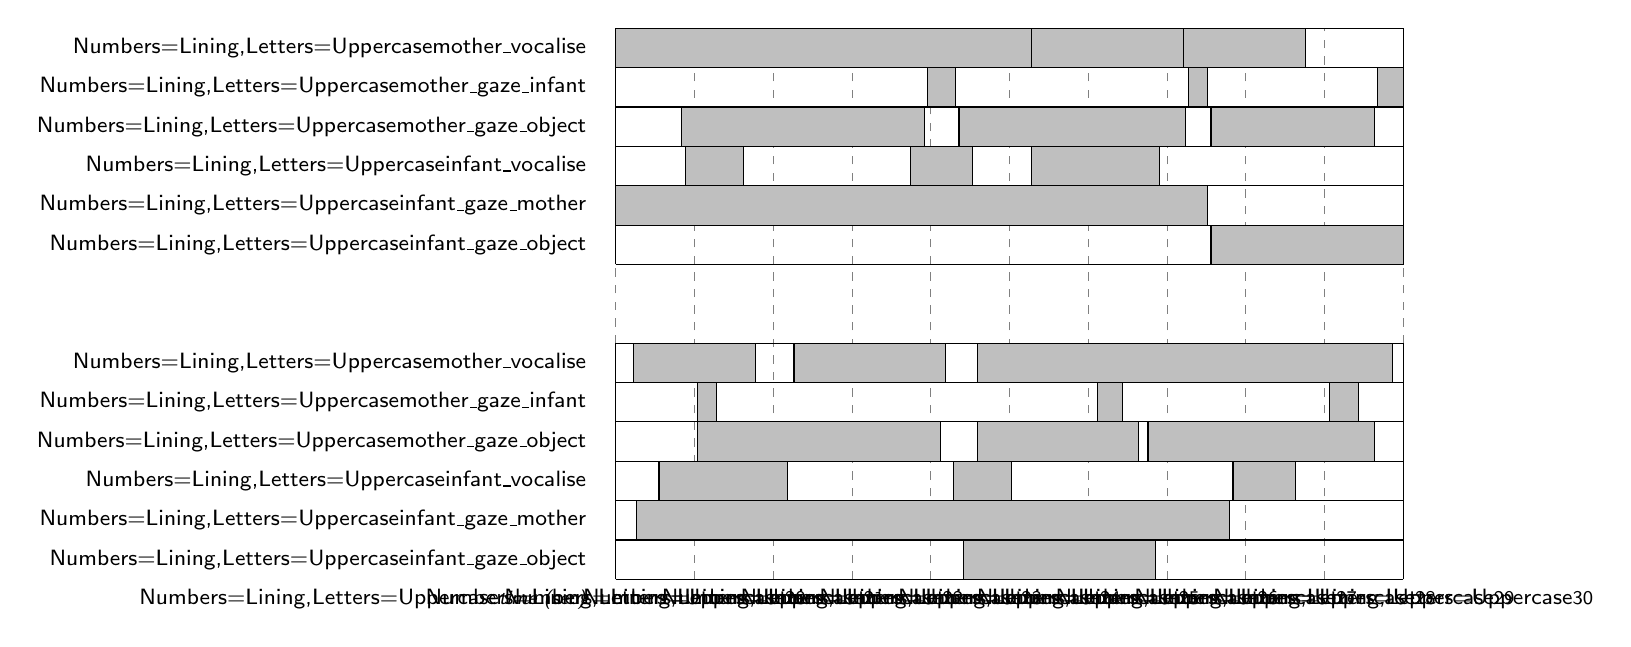
\begin{tikzpicture}[
	node distance=0 and 0,  % y, x for fuck knows what reason
	every node/.append style={font=\footnotesize\sffamily\addfontfeature{Numbers=Lining,Letters=Uppercase}}]
%	\draw [help lines, dashed] (0,0) grid (13,7);
	
	% time line
	% annotations
	\node [anchor=east] at (2.75, -0.25) {\textit{\scriptsize{time (sec)}}};
	\foreach \i in {20, 21,..., 29, 30}
		\node at ({\i-17},-0.25) {\scriptsize{\i}};
	% small vertical help lines
	\draw [help lines, dashed] (3,3) -- (3,4);
	\draw [help lines, dashed] (13,3) -- (13,4);
	% long vertical help lines
	\foreach \i in {4, 5,..., 11, 12}
		\draw [help lines, dashed] (\i,0) -- (\i,7);
	
	%% grids
	% vertical lines
	\foreach \i in {3, 13}{
		\draw (\i,4) -- (\i,7);  % top
		\draw (\i,0) -- (\i,3);  % bottom
	}
	% horizontal lines
	\foreach \i in {0, 0.5,..., 2.5, 3, 4, 4.5,..., 6.5, 7}  % top and bottom
		\draw (3,\i) -- (13,\i);
%	% annotations, not happy with them the way they are
%	\node[rotate=-90, anchor=south] at (13,5.5) {\textsc{real}};
%	\node[rotate=-90, anchor=south] at (13,1.5) {\textsc{null}};
		
	%% labels
	\foreach \i in {0.25, 4.25}{  % top and bottom
		\node[anchor=east] at (2.75,{\i+2.5}) {\code{mother\_vocalise}};
		\node[anchor=east] at (2.75,{\i+2}) {\code{mother\_gaze\_infant}};
		\node[anchor=east] at (2.75,{\i+1.5}) {\code{mother\_gaze\_object}};
		\node[anchor=east] at (2.75,{\i+1}) {\code{infant\_vocalise}};
		\node[anchor=east] at (2.75,{\i+0.5}) {\code{infant\_gaze\_mother}};
		\node[anchor=east] at (2.75,\i) {\code{infant\_gaze\_object}};
	}
	
	%% annotations
	% top
	\draw [fill=lightgray] (3,6.5) rectangle (8.279,7);
	\draw [fill=lightgray] (8.279,6.5) rectangle (10.206,7);
	\draw [fill=lightgray] (10.206,6.5) rectangle (11.76,7);

	\draw [fill=lightgray] (6.96,6) rectangle (7.32,6.5);
	\draw [fill=lightgray] (10.28,6) rectangle (10.52,6.5);
	\draw [fill=lightgray] (12.68,6) rectangle (13,6.5);
	
	\draw [fill=lightgray] (3.84,5.5) rectangle (6.92,6);
	\draw [fill=lightgray] (7.36,5.5) rectangle (10.24,6);
	\draw [fill=lightgray] (10.56,5.5) rectangle (12.64,6);
	
	\draw [fill=lightgray] (3.887,5) rectangle (4.624,5.5);
	\draw [fill=lightgray] (6.74,5) rectangle (7.53,5.5);
	\draw [fill=lightgray] (8.279,5) rectangle (9.909,5.5);
	
	\draw [fill=lightgray] (3,4.5) rectangle (10.52,5);

	\draw [fill=lightgray] (10.56,4) rectangle (13,4.5);
	% bottom
	\draw [fill=lightgray] (7.592,2.5) rectangle (12.871,3);
	\draw [fill=lightgray] (5.264,2.5) rectangle (7.191,3);
	\draw [fill=lightgray] (3.221,2.5) rectangle (4.775,3);

	\draw [fill=lightgray] (12.069,2) rectangle (12.429,2.5);
	\draw [fill=lightgray] (4.039,2) rectangle (4.279,2.5);
	\draw [fill=lightgray] (9.115,2) rectangle (9.435,2.5);
	
	\draw [fill=lightgray] (4.04,1.5) rectangle (7.12,2);
	\draw [fill=lightgray] (9.76,1.5) rectangle (12.64,2);
	\draw [fill=lightgray] (7.59,1.5) rectangle (9.64,2);
	
	\draw [fill=lightgray] (7.287,1) rectangle (8.024,1.5);
	\draw [fill=lightgray] (10.84,1) rectangle (11.63,1.5);
	\draw [fill=lightgray] (3.55,1) rectangle (5.18,1.5);
	
	\draw [fill=lightgray] (3.27,0.5) rectangle (10.79,1);

	\draw [fill=lightgray] (7.42,0) rectangle (9.86,0.5);
\end{tikzpicture}
	\caption{fig:nullnaive}
	\label{fig:nullnaive}
\end{figure}

\begin{figure}
	\centering
	% !TEX root = ../../scrreprt/ba_scrreprt_master.tex
% @author Marcel Ruland (2018)

\begin{tikzpicture}
	[every node/.append style={font=\sffamily\addfontfeature{Numbers=Lining,Letters=Uppercase}},
	rounded corners,
	align=center,
	>=stealth']
	
	% nodes
	\node [draw]						(chsig)	{Chapter \ref{ch:significance}};
	\node [draw, above left=of chsig]	(origin)	{\citeauthor{rohlfing18}};
	\node [draw, above right=of chsig]	(chmining)	{Chapter \ref{ch:mining}};
		
	% arrows
	\draw [->] (origin)			-- node[above]	{\footnotesize consider reaction times}		(chmining);
	\draw [->] (origin.south)	-- node[left]	{\footnotesize establish significance~~}	(chsig.west);
	\draw [->] (chmining.south)	-- node[right]	{\footnotesize ~~establish significance}	(chsig.east);
\end{tikzpicture}















































	\caption{fig:organisation}
	\label{fig:organisation}
\end{figure}

\begin{figure}
	\centering
	% !TEX root = ../../scrreprt/ba_scrreprt_master.tex
% @author Marcel Ruland (2018)

% semantic commands
\newcommand{\nullnode}{100 Null}
\newcommand{\samplenode}{sample}
\newcommand{\commentfont}[1]{{\rmfamily\tiny\textit{#1}}}
\newcommand{\annotationcounter}[1]{{\rmfamily\addfontfeature{Numbers=Lining}\scriptsize\textbf{#1.~}}}

% coordinates
\newcommand{\nully}{8}			% y-position of null nodes
\newcommand{\sampley}{5}		% y-position of sample nodes
\newcommand{\realx}{6}			% x position of leftmost real node
\newcommand{\realy}{\sampley}	% y-position of real nodes

% incrementers
\newcommand{\nullinc}{1.5}			% increment for null nodes
\newcommand{\sampleinc}{2}		% increment for sample nodes
\newcommand{\realinc}{1}			% increment for real nodes
\newcommand{\realtonullinc}{0.3}	% increment for real to null arrows

% other
\newcommand{\nodeoffset}{0.5}			% offset for \cdots
\newcommand{\annotationwidth}{1.5cm}	% width of annotations on left side
% gaussian function for plot
\pgfmathdeclarefunction{gauss}{2}{\pgfmathparse{1/(#2*sqrt(2*pi))*exp(-((x-#1)^2)/(2*#2^2))}}

\begin{tikzpicture}[
	every node/.append style={
		font=\sffamily\scriptsize\addfontfeature{
%			Numbers=Monospaced,
			Numbers=Lining,
			Letters=Uppercase
		}
	},
	node distance = 1 and 0.5,
	align=center
]
	% help lines
%	\draw[help lines, dashed] (0,0) grid (10,10);
	
	
	%%% NODES
	% null nodes
	\node[draw] at ({0 + 0*\nullinc},\nully)   (null1)  {\nullnode \\ 1};
	\node[draw] at ({0 + 1*\nullinc},\nully)   (null2)  {\nullnode \\ 2};
	\node[draw] at ({0 + 2*\nullinc},\nully)   (null3)  {\nullnode \\ 3};
	\node[draw] at ({0 + 3*\nullinc + \nodeoffset},\nully)   (null10) {\nullnode \\ 10};
	
	% sample nodes
	\node[draw] at ({0.5 + 0*\sampleinc},\sampley) (sample1) {\samplenode \\ 1};
	\node[draw] at ({0.5 + 1*\sampleinc},\sampley) (sample50) {\samplenode \\ 50};
	\node[draw] at ({0.5 + 2*\sampleinc},\sampley) (sample100) {\samplenode \\ 100};
	
	% real nodes
	\node[draw, circle, minimum size=2.5em] at ({\realx + 0*\realinc},\realy) (real1) {R1};
	\node[draw, circle, minimum size=2.5em] at ({\realx + 1*\realinc},\realy) (real2) {R2};
	\node[draw, circle, minimum size=2.5em] at ({\realx + 2*\realinc},\realy) (real3) {R3};
	\node[draw, circle, minimum size=2.5em] at ({\realx + 3*\realinc + \nodeoffset},\realy) (real10) {R10};
	
	% \cdots
	\path (null3) -- node{\(\cdots\)} (null10);
	\path (sample1) -- node{\(\cdots\)} (sample50);
	\path (sample50) -- node{\(\cdots\)} (sample100);
	\path (real3) -- node{\(\cdots\)} (real10);
	
	
	%%% ARROWS
	%% null to sample arrows
	% 1st sample
	\draw[-stealth, graphgreen] (null1.south west)  to (sample1.north);
	\draw[-stealth, graphgreen] (null2.south west)  to (sample1.north);
	\draw[-stealth, graphgreen] (null3.south west)  to (sample1.north);
	\draw[-stealth, graphgreen] (null10.south west) to (sample1.north);
	
	% 50th sample
	\draw[-stealth, graphgreen] (null1.south)  to (sample50.north);
	\draw[-stealth, graphgreen] (null2.south)  to (sample50.north);
	\draw[-stealth, graphgreen] (null3.south)  to (sample50.north);
	\draw[-stealth, graphgreen] (null10.south) to (sample50.north);
	
	% 100th sample
	\draw[-stealth, graphgreen] (null1.south east)  to (sample100.north);
	\draw[-stealth, graphgreen] (null2.south east)  to (sample100.north);
	\draw[-stealth, graphgreen] (null3.south east)  to (sample100.north);
	\draw[-stealth, graphgreen] (null10.south east) to (sample100.north);
	
	%% real to null arrows
	\draw[-stealth, graphred] (real1.north) to
					({\realx + 0*\realinc},{8.7 + 0*\realtonullinc}) to
					({0 + 0*\nullinc},{8.7 + 0*\realtonullinc}) to
					(null1.north);
					
	\draw[-stealth, graphred] (real2.north) to
					({\realx + 1*\realinc},{8.7 + 1*\realtonullinc}) to
					({0 + 1*\nullinc},{8.7 + 1*\realtonullinc}) to
					(null2.north);
					
	\draw[-stealth, graphred] (real3.north) to
					({\realx + 2*\realinc},{8.7 + 2*\realtonullinc}) to
					({0 + 2*\nullinc},{8.7 + 2*\realtonullinc}) to
					(null3.north);
					
	\draw[-stealth, graphred] (real10.north) to
					({\realx + 3*\realinc + \nodeoffset},{8.7 + 3*\realtonullinc}) to
					node[above, black]
					{\annotationcounter{1}\commentfont{generate 100 null distributions from each real sequence}}
					({0 + 3*\nullinc + \nodeoffset},{8.7 + 3*\realtonullinc}) to
					(null10.north);
	
	%% sample to plot arrows
	% nodes above plots
	\node[below=1.7cm of sample50.south] (greenplot) {};
	\node at (7.7,2.8) (redplot) {};
	
	% left plot
	\draw[-stealth, graphgreen] (sample1.south)  to (greenplot);
	\draw[-stealth, graphgreen] (sample50.south)  to (greenplot);
	\draw[-stealth, graphgreen] (sample100.south)  to (greenplot);
	
	% red plot
	\draw[-stealth, graphred] (real1.south)  to (redplot);
	\draw[-stealth, graphred] (real2.south)  to (redplot);
	\draw[-stealth, graphred] (real3.south)  to (redplot);
	\draw[-stealth, graphred] (real10.south)  to (redplot);
	
	
	
	%%% PLOTS
	%% left and green
	\begin{axis}[
		at={(110,0)},  % set origin coordinate in tikzpicture
		scale=0.5,  % half as large
		ymin=0,  % set ymin to 0
		xticklabels={,,},  % surpress digits at x-axis
		hide y axis,  % hide y axes (duh)
		axis x line*=bottom, % no box around the plot, only x and y axis
		every axis plot post/.append style={% All plots: from -2:2, 50 samples, smooth, no marks
			mark=none,
			domain=-2:2,
			samples=50,
			smooth
		}
	]
		% add normal curve
		\addplot[color=graphgreen] {gauss(0,0.5)};
		% add vertical line
		\draw[color=graphgreen, dashed] (axis cs:0,\pgfkeysvalueof{/pgfplots/ymin}) -- (axis cs:0,\pgfkeysvalueof{/pgfplots/ymax});
	\end{axis}
	
	%% right and red
	\begin{axis}[
		at={(1255,0)},  % set origin coordinate in tikzpicture
		scale=0.5,  % half as large
		ymin=0,  % set ymin to 0
		ymax=0.8,
		xticklabels={,,},  % surpress digits at x-axis
		hide y axis,  % hide y axes (duh)
		axis x line*=bottom, % no box around the plot, only x and y axis
		every axis plot post/.append style={% All plots: from -2:2, 50 samples, smooth, no marks
			mark=none,
			domain=-3:3,
			samples=50,
			smooth
		}
	]
		% add normal curve
		\addplot[color=graphred] {gauss(0,0.75)};
		% add vertical line
		\draw[color=graphred, dashed] (axis cs:0,\pgfkeysvalueof{/pgfplots/ymin}) -- (axis cs:0,\pgfkeysvalueof{/pgfplots/ymax});
	\end{axis}
	
	
	%%% THE BIG QUESTION
	\node at (5.1,0.7) (bigquestion) {\large\(\textcolor{graphgreen}{\mu_1} \stackrel{?}{=} \textcolor{graphred}{\mu_2}\)};
	
	%%% ANNOTATIONS
	% null to sample
	\draw[
		decorate,
		decoration={
			brace,
			amplitude=5pt
		}
	]
	([shift={(-0.6,0.025)}]sample1.north west) --
	([shift={(-0.1,0)}]null1.south west)
	node[
		midway,
		left,
		xshift=-0.5em,
		align=right,
		text width=\annotationwidth
	]
	{\annotationcounter{2}\commentfont{\emph{i}-th null distribution goes into \emph{i}-th sample}};
	
	% apply fpm
	\draw[
		decorate,
		decoration={
			brace,
			amplitude=5pt
		}
	]
	([shift={(-0.6,0.025)}]sample1.south west) --
	([shift={(-0.6,-0.025)}]sample1.north west)
	node[
		midway,
		left,
		xshift=-0.5em,
		align=right,
		text width=\annotationwidth
	]
	{\annotationcounter{3}\commentfont{apply \textsc{fpm} to all samples and real sequences separately}};
	
	% probability
	\draw[
		decorate,
		decoration={
			brace,
			amplitude=5pt
		}
	]
	([shift={(-0.1,0)}]-0.5,0) --
	([shift={(-0.6,-0.025)}]sample1.south west)
	node[
		midway,
		left,
		xshift=-0.5em,
		align=right,
		text width=\annotationwidth
	]
	{\annotationcounter{4}\commentfont{probabilities of rule \emph{i} from all samples form probability distribution of rule \emph{i}}};
	
	\node[
		above=0.2cm of bigquestion,
		align=left,
		text width=2.5cm
	]
	{\annotationcounter{5}\commentfont{test the real probability distribution for significance against the null probability distribution}};
	
	%%% HELP LINES (turned out to be ugly af)
%	\draw[dashed] (-0.6,0) to (10,0);
%	\draw[dashed] (-0.6,4.6) to (10,4.6);
%	\draw[dashed] (-0.6,5.4) to (10,5.4);
%	\draw[dashed] (-0.6,7.6) to (5.6,7.6);
\end{tikzpicture}
	\caption{fig:significance}
	\label{fig:significance}
\end{figure}


\end{document}
